\documentclass[11pt]{article}

\usepackage[margin=0.78in]{geometry}
\usepackage[T1]{fontenc}
\usepackage{lmodern}
\usepackage{microtype}
\usepackage{graphicx}
\usepackage{booktabs}
\usepackage{tabularx}
\usepackage{array}
\usepackage[table]{xcolor}
\usepackage{caption}
\usepackage{placeins}
\usepackage{float}
\usepackage{tikz}
\usepackage{pgfplots}
\usepackage{hyperref}
\usetikzlibrary{arrows.meta,positioning,calc}
\pgfplotsset{compat=1.18}

\definecolor{hitone}{RGB}{229,241,233}
\definecolor{hitfive}{RGB}{229,237,247}
\definecolor{inkblue}{RGB}{54,91,130}
\definecolor{inkorange}{RGB}{205,111,45}
\definecolor{inkgray}{RGB}{96,103,110}
\definecolor{lightgray}{RGB}{241,242,243}

\hypersetup{colorlinks=true,linkcolor=black,urlcolor=black}
\newcolumntype{Y}{>{\raggedright\arraybackslash}X}
\newcolumntype{L}[1]{>{\raggedright\arraybackslash}p{#1}}
\newcolumntype{R}[1]{>{\raggedleft\arraybackslash}p{#1}}
\newcolumntype{G}{>{\columncolor{hitone}\raggedleft\arraybackslash}p{0.09\linewidth}}
\newcolumntype{B}{>{\columncolor{hitfive}\raggedleft\arraybackslash}p{0.09\linewidth}}
\newcolumntype{N}{>{\raggedleft\arraybackslash}p{0.09\linewidth}}
\newcommand{\code}[1]{\texttt{#1}}

\setlength{\parindent}{0pt}
\setlength{\parskip}{0.38em}
\renewcommand{\arraystretch}{1.12}
\captionsetup{font=small,labelfont=bf}
\clubpenalty=10000
\widowpenalty=10000

\title{\textbf{Algorithms 1--6: Results and Decision Logic}\\
\large A compact benchmark briefing}
\author{medicine-search-clean}
\date{4 August 2026}

\begin{document}
\maketitle

\begin{abstract}
The comparison uses 464 fair OCR query--target pairs and 66,257 clean synthetic
cases. Algorithm 6 reaches 50.43\% Hit@1, 63.58\% Hit@5, and 73.28\% Hit@20 on
OCR. It has the same Hit@1 and Hit@5 as Algorithm 5, but retrieves two additional
OCR targets at rank 20. A broader rule that changed rank 1 was rejected because
it gained 27 synthetic cases and lost 138.
\end{abstract}

\section{Read the Numbers First}

A \textbf{medicine family} is the commercial-name group being ranked. A
\textbf{candidate} is one family shown to the user. A \textbf{retrieval source}
is one search method that independently returns a ranked candidate list.

\begin{table}[htbp]
\centering
\small
\begin{tabularx}{\linewidth}{@{}L{0.20\linewidth}rGNBNR{0.14\linewidth}@{}}
\toprule
\textbf{Dataset} & \textbf{Cases} & \textbf{Hit@1} & \textbf{Correct} & \textbf{Hit@5} & \textbf{Correct} & \textbf{Hit@20} \\
\midrule
Fair OCR pairs & 464 & 50.43\% & 234 & 63.58\% & 295 & 73.28\% (340) \\
Synthetic clean core & 66,257 & 98.19\% & 65,057 & 99.65\% & 66,027 & 99.9985\% (66,256) \\
\bottomrule
\end{tabularx}
\caption{Algorithm 6 headline counts. Hit@1 means the expected family is first;
Hit@5 and Hit@20 mean it appears within the first five or twenty families. The
green and blue columns identify Hit@1 and Hit@5 throughout the report.}
\label{tab:headline}
\end{table}

The OCR set gives one vote to each unique fair query--target pair. The synthetic
set applies generated spelling errors to catalog-derived targets and excludes
unfair cases where the corrupted query is exactly another real family name.

\section{What Changed from Algorithm 1 to Algorithm 6}

The algorithm names are their version numbers. The descriptions below explain
the change; they are not additional algorithm names.

\begin{table}[htbp]
\centering
\small
\begin{tabularx}{\linewidth}{@{}L{0.14\linewidth}Y R{0.13\linewidth}@{}}
\toprule
\textbf{Algorithm} & \textbf{Change introduced in that version} & \textbf{OCR ms/query} \\
\midrule
Algorithm 1 & Original application search over medicine names. & 1.28 \\
Algorithm 2 & Independent fast typo search that narrows the catalog before comparison. & 4.75 \\
Algorithm 3 & Combines the ranked lists produced by Algorithms 1 and 2. & 6.84 \\
Algorithm 4 & Adds family and visible-fragment recovery for longer product names. & 14.89 \\
Algorithm 5 & Adds position, missing-letter, sound, and family evidence learned from failure analysis. & 28.54 \\
Algorithm 6 & Keeps Algorithm 5's order and may add one independently supported missing family at rank 20. & 48.50 \\
\bottomrule
\end{tabularx}
\caption{Each version adds a specific capability and increases mean OCR query
time. Algorithm 6 does not replace Algorithm 5's first result.}
\label{tab:versions}
\end{table}

\begin{table}[htbp]
\centering
\small
\setlength{\tabcolsep}{4pt}
\begin{tabularx}{\linewidth}{@{}YGBNGBN@{}}
\toprule
& \multicolumn{3}{c}{\textbf{464 fair OCR pairs}} & \multicolumn{3}{c}{\textbf{66,257 synthetic pairs}} \\
\cmidrule(lr){2-4}\cmidrule(lr){5-7}
\textbf{Method} & \textbf{H@1} & \textbf{H@5} & \textbf{H@20} & \textbf{H@1} & \textbf{H@5} & \textbf{H@20} \\
\midrule
Algorithm 1 & 23.71 & 31.47 & 38.15 & 83.86 & 89.72 & 92.23 \\
Algorithm 2 & 25.86 & 43.75 & 51.29 & 92.41 & 96.33 & 96.88 \\
Algorithm 3 & 25.65 & 40.95 & 53.02 & 91.84 & 96.18 & 97.12 \\
Algorithm 4 & 47.63 & 61.85 & 71.12 & 97.19 & 99.24 & 99.52 \\
Algorithm 5 & \textbf{50.43} & \textbf{63.58} & 72.84 & \textbf{98.19} & \textbf{99.65} & \textbf{99.9985} \\
Algorithm 6 & \textbf{50.43} & \textbf{63.58} & \textbf{73.28} & \textbf{98.19} & \textbf{99.65} & \textbf{99.9985} \\
\bottomrule
\end{tabularx}
\caption{Percent recovery. Algorithm 6 improves Algorithm 5 only at Hit@20:
340 rather than 338 OCR pairs.}
\label{tab:project-results}
\end{table}

\begin{table}[htbp]
\centering
\small
\setlength{\tabcolsep}{4pt}
\begin{tabularx}{\linewidth}{@{}YGBNGBN@{}}
\toprule
& \multicolumn{3}{c}{\textbf{464 fair OCR pairs}} & \multicolumn{3}{c}{\textbf{66,257 synthetic pairs}} \\
\cmidrule(lr){2-4}\cmidrule(lr){5-7}
\textbf{Method} & \textbf{H@1} & \textbf{H@5} & \textbf{H@20} & \textbf{H@1} & \textbf{H@5} & \textbf{H@20} \\
\midrule
SymSpell, edit distance 3 & 38.58 & 50.86 & 55.82 & 94.22 & 98.08 & 98.80 \\
Damerau--Levenshtein & 34.27 & 50.65 & 59.27 & 94.78 & 98.69 & 99.64 \\
Exhaustive Levenshtein & 34.27 & 50.86 & 59.27 & 94.05 & 98.40 & 99.44 \\
Jaro--Winkler & 32.11 & 55.17 & 67.46 & 89.57 & 96.26 & 98.43 \\
BM25+ character trigrams & 20.26 & 35.13 & 47.41 & 78.19 & 87.79 & 92.17 \\
BioSyn-style hybrid & 19.40 & 39.66 & 50.86 & 77.88 & 88.88 & 93.40 \\
Character 3-gram TF--IDF & 18.32 & 35.78 & 47.41 & 75.21 & 86.72 & 91.66 \\
xMEN-style dense+sparse fusion & 16.81 & 37.50 & 52.37 & 48.85 & 78.51 & 92.30 \\
SapBERT dense retrieval & 11.42 & 22.63 & 38.58 & 27.67 & 44.00 & 56.45 \\
RapidFuzz weighted ratio & 11.21 & 40.30 & 56.25 & 55.73 & 93.49 & 97.20 \\
Phonetic baseline & 6.90 & 16.81 & 23.28 & 69.66 & 84.92 & 92.07 \\
Exact or prefix match & 2.59 & 2.80 & 3.02 & 3.00 & 3.01 & 3.01 \\
\bottomrule
\end{tabularx}
\caption{Percent recovery for the main non-project method families. The same
input, catalog, family-level scoring, and denominator are used for every row.}
\label{tab:external-results}
\end{table}

\begin{figure}[htbp]
\centering
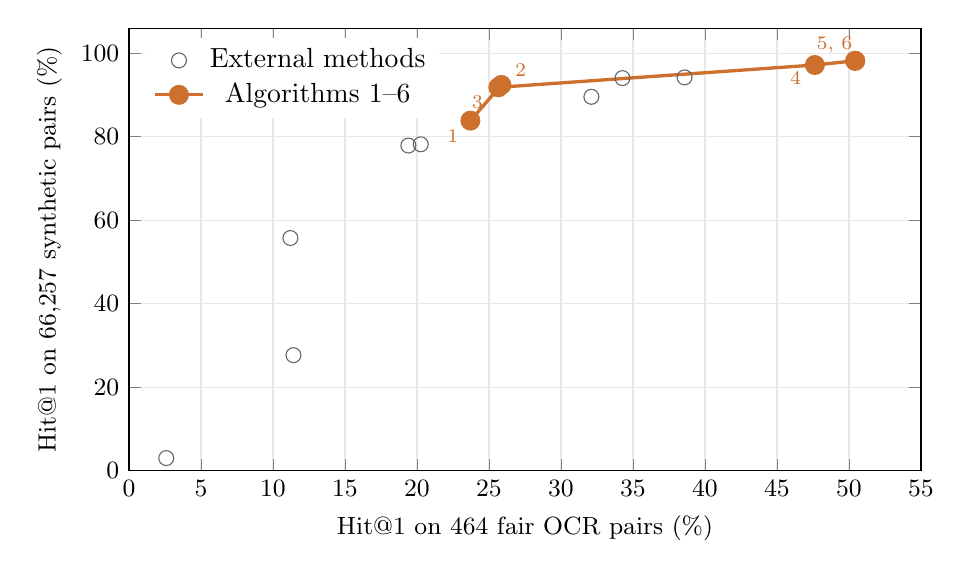
\begin{tikzpicture}
\begin{axis}[
  width=0.96\linewidth,
  height=7.2cm,
  xmin=0,xmax=55,
  ymin=0,ymax=106,
  xlabel={Hit@1 on 464 fair OCR pairs (\%)},
  ylabel={Hit@1 on 66,257 synthetic pairs (\%)},
  grid=major,
  grid style={draw=gray!18},
  legend style={at={(0.02,0.98)},anchor=north west,draw=none},
  tick label style={font=\small},
  label style={font=\small}
]
\addplot[only marks,mark=o,mark size=2.7pt,color=inkgray] coordinates {
  (2.59,3.00) (34.27,94.05) (32.11,89.57) (38.58,94.22)
  (19.40,77.88) (11.42,27.67) (20.26,78.19) (11.21,55.73)
};
\addlegendentry{External methods}
\addplot[color=inkorange,very thick,mark=*,mark size=3pt] coordinates {
  (23.71,83.86) (25.86,92.41) (25.65,91.84)
  (47.63,97.19) (50.43,98.19) (50.43,98.19)
};
\addlegendentry{Algorithms 1--6}
\node[font=\scriptsize,text=inkorange] at (axis cs:22.5,80.0) {1};
\node[font=\scriptsize,text=inkorange] at (axis cs:27.2,96.0) {2};
\node[font=\scriptsize,text=inkorange] at (axis cs:24.2,88.2) {3};
\node[font=\scriptsize,text=inkorange] at (axis cs:46.3,94.0) {4};
\node[font=\scriptsize,text=inkorange] at (axis cs:49.0,102.0) {5, 6};
\end{axis}
\end{tikzpicture}
\caption{Each point uses OCR Hit@1 on the x-axis and synthetic Hit@1 on the
y-axis. Numbers beside orange points identify Algorithms 1--6. Synthetic
results are much higher for nearly every method, so the 66,257-case score cannot
replace OCR evaluation. Algorithms 5 and 6 occupy the same point because
Algorithm 6 does not change rank 1.}
\label{fig:cross-dataset}
\end{figure}

\FloatBarrier
\section{Where the Remaining Retrieval Problem Starts}

Compact edit distance counts the fewest single-character insertions, deletions,
or replacements after case, spaces, and punctuation are removed. For example,
\code{TEFA}$\rightarrow$\code{TELFAST} needs three insertions.

\begin{figure}[htbp]
\centering
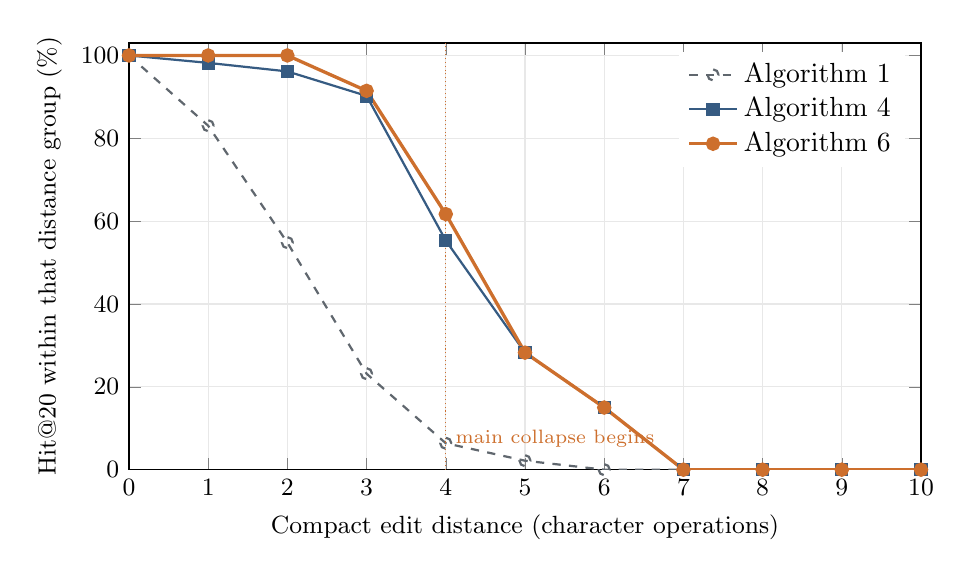
\begin{tikzpicture}
\begin{axis}[
  width=0.96\linewidth,
  height=7.0cm,
  xmin=0,xmax=10,
  ymin=0,ymax=103,
  xtick={0,1,2,3,4,5,6,7,8,9,10},
  xlabel={Compact edit distance (character operations)},
  ylabel={Hit@20 within that distance group (\%)},
  grid=major,
  grid style={draw=gray!18},
  legend style={at={(0.98,0.98)},anchor=north east,draw=none},
  tick label style={font=\small},
  label style={font=\small}
]
\addplot[color=inkgray,dashed,thick,mark=o] coordinates {
  (0,100) (1,83.04) (2,54.81) (3,23.17) (4,6.38) (5,2.17)
  (6,0) (7,0) (8,0) (9,0) (10,0)
};
\addlegendentry{Algorithm 1}
\addplot[color=inkblue,thick,mark=square*] coordinates {
  (0,100) (1,98.21) (2,96.15) (3,90.24) (4,55.32) (5,28.26)
  (6,15.00) (7,0) (8,0) (9,0) (10,0)
};
\addlegendentry{Algorithm 4}
\addplot[color=inkorange,very thick,mark=*] coordinates {
  (0,100) (1,100) (2,100) (3,91.46) (4,61.70) (5,28.26)
  (6,15.00) (7,0) (8,0) (9,0) (10,0)
};
\addlegendentry{Algorithm 6}
\draw[densely dotted,inkorange] (axis cs:4,0) -- (axis cs:4,103);
\node[font=\scriptsize,anchor=south west,text=inkorange] at (axis cs:4,3) {main collapse begins};
\end{axis}
\end{tikzpicture}
\caption{The x-axis is corruption severity and the y-axis is retrieval within
the first 20. Algorithm 6 retrieves every one- and two-edit OCR case, 91.46\%
of three-edit cases, 61.70\% at four edits, and none at seven or more. The next
retrieval work should target four-to-six-edit evidence rather than easy typos.}
\label{fig:distance}
\end{figure}

\section{How Algorithm 6 Makes One Decision}

Algorithm 6 starts with Algorithm 5's top 20. Nine additional methods search
the same catalog. Names referring to the same family are merged. A family absent
from Algorithm 5's list can enter only the final slot when all three rules pass:

\begin{enumerate}
  \item at least three retrieval sources return it;
  \item Levenshtein similarity is at least 55\%;
  \item Jaro--Winkler similarity is at least 85\%.
\end{enumerate}

Levenshtein similarity is $1-d/\max(|q|,|c|)$, where $d$ is edit distance,
$q$ is the query, and $c$ is the candidate. Jaro--Winkler is a 0--1 score that
rewards matching characters in the same order and gives extra weight to a
shared prefix. Algorithm 6 adds at most one family at rank 20 and never changes
rank 1.

Algorithm 5 is not one opaque component inside Algorithm 6. It is the complete
base pipeline summarized below. Algorithm 6 then adds the independent sources,
family-level consensus, bounded insertion gate, and confirmation policy.

\begin{table}[htbp]
\centering
\small
\begin{tabularx}{\linewidth}{@{}L{0.20\linewidth}L{0.27\linewidth}Y@{}}
\toprule
\textbf{Nested Algorithm 5 component} & \textbf{Cases it handles} & \textbf{Concrete benchmark example} \\
\midrule
Normalization and context cleanup & Case, punctuation, spacing, strength, route, and form text around a name. & \code{AAPE RENEWAL SUNSCREEN SPF 60ML}$\rightarrow$\code{AAPE RENEWAL SUNSCREEN SPF}. \\
External candidate retriever & Broad typo candidates and a second pass after context cleanup. & Removing it loses \code{ABDUSONG LAR}$\rightarrow$\code{ABASAGLAR} from Algorithm 6's top 20. \\
Family-rescue index & Exact, prefix, suffix, character n-gram, consonant, phonetic, delete-key, and compatible-length lookup over 17,476 families. & \code{MYMLAX}$\rightarrow$\code{MYOLAX} survives a middle-character substitution. \\
String-evidence scores & Raw and weighted edit similarity, prefix, suffix, n-grams, phonetic code, skeleton, subsequence, position, and length coverage. & \code{TEFAXATE}$\rightarrow$\code{TELFAST} uses position and shared-edge evidence. \\
Error-variant retrieval & Keyboard, ligature, transposition, visual, phonetic, missing-letter, and bounded multi-step transformations. & Synthetic \code{uraranx}$\rightarrow$\code{ORAMAX} depends on the multi-step family in the non-regression set. \\
Family-head and short-fragment rescue & Matches visible family heads and short prefix/suffix evidence without treating every substring as decisive. & \code{LANS}$\rightarrow$\code{LANTUS} is lost from top 20 when short visible-head rescue is removed. \\
Deterministic rerankers & Correct equal-distance and evidence-dominance cases after candidate merging. & \code{LANYU}$\rightarrow$\code{LANTUS} falls outside top 20 when all rerankers are removed. \\
Clarification gate & Keeps the ranking but marks weak, short, or conflicting evidence for user confirmation. & \code{RIV}$\rightarrow$\code{RIVOTRIL} competes with the shorter catalog family \code{RIVO}; the system must not certify one answer. \\
\bottomrule
\end{tabularx}
\caption{The internal Algorithm 5 pipeline that Algorithm 6 executes first.
The later ablation removes these components inside Algorithm 6 and then leaves
all nine additional sources and the consensus gate active.}
\label{tab:a6-nested-a5-components}
\end{table}

\begin{figure}[htbp]
\centering
\resizebox{\linewidth}{!}{%
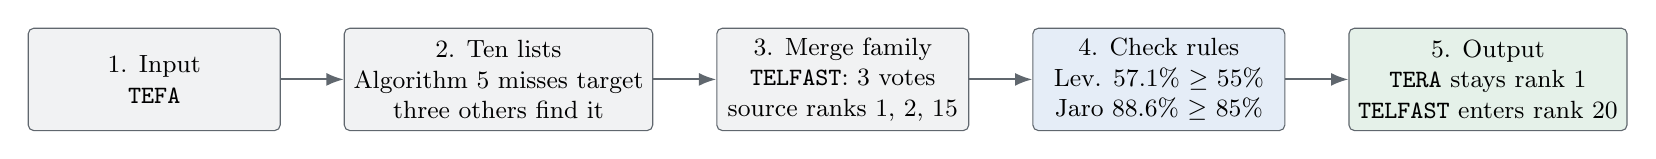
\begin{tikzpicture}[
  node distance=8mm,
  box/.style={rectangle,draw=inkgray,rounded corners=2pt,align=center,
              minimum height=13mm,minimum width=32mm,font=\small},
  arrow/.style={-{Latex[length=2.2mm]},draw=inkgray,line width=0.7pt}
]
\node[box,fill=lightgray] (input) {1. Input\\\code{TEFA}};
\node[box,fill=lightgray,right=of input] (lists) {2. Ten lists\\Algorithm 5 misses target\\three others find it};
\node[box,fill=lightgray,right=of lists] (merge) {3. Merge family\\\code{TELFAST}: 3 votes\\source ranks 1, 2, 15};
\node[box,fill=hitfive,right=of merge] (gate) {4. Check rules\\Lev. 57.1\% $\geq$ 55\%\\Jaro 88.6\% $\geq$ 85\%};
\node[box,fill=hitone,right=of gate] (output) {5. Output\\\code{TERA} stays rank 1\\\code{TELFAST} enters rank 20};
\draw[arrow] (input) -- (lists);
\draw[arrow] (lists) -- (merge);
\draw[arrow] (merge) -- (gate);
\draw[arrow] (gate) -- (output);
\end{tikzpicture}%
}
\caption{Complete decision for \code{TEFA}. The hidden benchmark target is
\code{TELFAST}, but it is never shown to search. Independent lists provide the
three votes; the two similarity checks pass; the candidate is added at rank 20.
The top result remains \code{TERA}, so the interface must request confirmation.}
\label{fig:decision-flow}
\end{figure}

\begin{table}[htbp]
\centering
\small
\begin{tabularx}{\linewidth}{@{}L{0.20\linewidth}L{0.25\linewidth}L{0.27\linewidth}Y@{}}
\toprule
\textbf{Retrieval source} & \textbf{What it measures} & \textbf{Actual case it retrieves} & \textbf{Measured role} \\
\midrule
Algorithm 5 & Complete base pipeline above & \code{MYMLAX}$\rightarrow$\code{MYOLAX} at rank 1 & Preserves all deployed rank-1 ordering. \\
Jaro--Winkler & Character order and shared prefix & \code{TEFA}$\rightarrow$\code{TELFAST} at source rank 1 & Required for the \code{TEFA} top-20 gain. \\
Match Rating & Compressed consonant pattern & \code{ABASCOLOGY}$\rightarrow$\code{ABASAGLAR} at source rank 1 & No isolated top-$k$ change on 464 OCR pairs. \\
RapidFuzz weighted ratio & Best direct or partial string ratio & \code{LACTULOSE}$\rightarrow$\code{LACTO} at source rank 3 & Supports \code{LACTO}; redundant under one-source removal. \\
NYSIIS & Pronunciation-oriented code & \code{MYOLOGY}$\rightarrow$\code{MYOLAX} at source rank 1 & No isolated top-$k$ change on 464 OCR pairs. \\
BM25+ trigrams & Weighted shared three-character pieces & \code{LACTULOSE}$\rightarrow$\code{LACTO} at source rank 12 & Required to select the \code{LACTO} gain over another outside candidate. \\
SymSpell & Candidates within three delete-key edits & \code{OSFOCU}$\rightarrow$\code{OSTOCAL} at source rank 1 & No isolated top-$k$ change on 464 OCR pairs. \\
RapidFuzz token-sort & Token/string comparison after normalization & \code{TEFA}$\rightarrow$\code{TELFAST} at rank 2; \code{LACTULOSE}$\rightarrow$\code{LACTO} at rank 5 & Removing it loses one deployed gain. \\
Soundex & Coarse first-letter and consonant sound & \code{TELBACE}$\rightarrow$\code{TELFAST} at source rank 1 & Broad phonetic backstop; never sufficient alone. \\
Dice bigrams & Shared two-character pieces & \code{TEFA}$\rightarrow$\code{TELFAST} at source rank 15 & Supplies \code{TEFA}'s third required vote. \\
\bottomrule
\end{tabularx}
\caption{Every candidate source is tied to an actual benchmark row. ``No
isolated change'' means the remaining sources preserved the same top-$k$
outcome on this sample; it does not mean the source never retrieves useful
candidates.}
\label{tab:source-evidence}
\end{table}

\begin{table}[htbp]
\centering
\small
\begin{tabularx}{\linewidth}{@{}L{0.15\linewidth}L{0.15\linewidth}rrrrY@{}}
\toprule
\textbf{Input} & \textbf{Supplied target} & \textbf{Sources} & \textbf{Lev.} & \textbf{Jaro} & \textbf{A5 $\rightarrow$ A6 rank} & \textbf{Unchanged top 1} \\
\midrule
\code{TEFA} & \code{TELFAST} & 3 & 57.1\% & 88.6\% & $>20\rightarrow20$ & \code{TERA} \\
\code{LACTULOSE} & \code{LACTO} & 5 & 55.6\% & 91.1\% & $>20\rightarrow20$ & \code{LACTULOSE HEK} \\
\bottomrule
\end{tabularx}
\caption{Both rows pass the three-source and two-similarity rules. They are P0
and P1 audit cases, so they prove a retrieval change, not that the supplied
target is clinically or visually correct. Source-crop review is still required.}
\label{tab:gain-examples}
\end{table}

\FloatBarrier
\section{Ablation: What Actually Contributes}

A true Algorithm 6 ablation removes one component, reruns the changed Algorithm
5 base, and then executes the other nine retrieval sources and the same
consensus gate. It does not copy an Algorithm 5-only percentage. A
percentage-point change is absolute: 73.276\% to 72.845\% is $-0.431$ points.
``G/L'' reports paired gains and losses relative to complete Algorithm 6.

\begin{table}[htbp]
\centering
\scriptsize
\setlength{\tabcolsep}{3.2pt}
\begin{tabularx}{\linewidth}{@{}YrrrrrL{0.25\linewidth}@{}}
\toprule
\textbf{Nested component removed} & \textbf{H@1} & \textbf{$\Delta$H@1} & \textbf{H@20} & \textbf{$\Delta$H@20} & \textbf{H@20 G/L} & \textbf{Actual affected case} \\
\midrule
Family rescue & 36.638 & $-13.793$ & 56.034 & $-17.241$ & 3/83 & \code{TUTORIALAE}$\rightarrow$\code{KETOROLAC}: rank 7 to $>20$. \\
All deterministic reranking & 40.517 & $-9.914$ & 70.690 & $-2.586$ & 0/12 & \code{LANYU}$\rightarrow$\code{LANTUS}: rank 2 to $>20$. \\
Weighted edit similarity & 49.569 & $-0.862$ & 66.164 & $-7.112$ & 2/35 & The largest scoring-signal loss at top 20. \\
Raw edit similarity & 49.353 & $-1.078$ & 67.888 & $-5.388$ & 2/27 & Removes the uniform character-distance score. \\
Short-edge retrieval & 49.784 & $-0.647$ & 70.259 & $-3.017$ & 0/14 & \code{RICOHIL}$\rightarrow$\code{RIVOTRIL}: rank 3 to $>20$. \\
Length coverage & 50.216 & $-0.216$ & 70.259 & $-3.017$ & 1/15 & Penalizes candidates whose visible-length support is weak. \\
Family-head rescue & 48.060 & $-2.371$ & 70.905 & $-2.371$ & 0/11 & \code{LANYU}$\rightarrow$\code{LANTUS}: rank 2 to $>20$. \\
Delete-key retrieval & 48.276 & $-2.155$ & 71.121 & $-2.155$ & 0/10 & Recovers names explained by missing characters. \\
Prefix evidence & 48.707 & $-1.724$ & 71.336 & $-1.940$ & 0/9 & \code{RIVITAM}$\rightarrow$\code{RIVOTRIL}: rank 17 to $>20$. \\
Positional evidence & 48.922 & $-1.509$ & 71.336 & $-1.940$ & 1/10 & \code{TEFAXATE}$\rightarrow$\code{TELFAST}: rank 16 to $>20$. \\
Character n-grams & 48.060 & $-2.371$ & 71.983 & $-1.293$ & 2/8 & Local character pieces retain evidence around OCR errors. \\
External retriever & 49.784 & $-0.647$ & 72.414 & $-0.862$ & 0/4 & \code{ABDUSONG LAR}$\rightarrow$\code{ABASAGLAR}: rank 1 to $>20$. \\
Weighted confusion costs & 48.707 & $-1.724$ & 72.845 & $-0.431$ & 3/5 & \code{KETOMAN}$\rightarrow$\code{KATOMOR}: rank 14 to $>20$. \\
Phonetic evidence & 49.569 & $-0.862$ & 73.276 & $0.000$ & 0/0 & \code{ECOFIXIM}$\rightarrow$\code{CEFIXIME}: rank 1 falls to rank 2. \\
Short visible-head rescue & 50.431 & $0.000$ & 73.060 & $-0.216$ & 0/1 & \code{LANS}$\rightarrow$\code{LANTUS}: rank 20 to $>20$. \\
\bottomrule
\end{tabularx}
\caption{End-to-end OCR ablations over the same 464 pairs. Algorithm 6 remains
active after each nested removal, so its independent sources may recover cases
lost by the modified base. Gains and losses are not additive because several
components can affect the same row.}
\label{tab:nested-a6-ablation}
\end{table}

The complete CSV contains 96 nested removals, including atomic flags. Two
cross-dataset results change the interpretation. Removing all multi-step chains
has zero OCR top-$k$ effect because other sources cover the same OCR rows, but
loses 343 synthetic Hit@1 cases while gaining 3, and loses 178 synthetic Hit@20
cases with no gains. Removing
family-head rescue loses 11 OCR Hit@20 cases but gains 22 net synthetic Hit@1
cases and recovers the single synthetic top-20 miss, \code{aclox}$\rightarrow$
\code{ADOX}. That conflict needs a narrower guard, not deletion of the whole
component.

\begin{table}[htbp]
\centering
\small
\begin{tabularx}{\linewidth}{@{}L{0.25\linewidth}rrrY@{}}
\toprule
\textbf{Algorithm 6 component removed} & \textbf{OCR H@20} & \textbf{Cases lost} & \textbf{$\Delta$H@20} & \textbf{Why} \\
\midrule
Bounded rank-20 slot & 72.845\% & 2 & $-0.431$ pp & Both \code{TEFA} and \code{LACTULOSE} return outside the top 20. \\
Jaro--Winkler & 73.060\% & 1 & $-0.216$ pp & \code{TELFAST} falls below three supporting sources. \\
RapidFuzz token-sort & 73.060\% & 1 & $-0.216$ pp & The same \code{TEFA} case loses one required vote. \\
Dice bigrams & 73.060\% & 1 & $-0.216$ pp & Shared pieces \code{TE} and \code{FA} supplied the third vote. \\
BM25+ trigrams & 73.060\% & 1 & $-0.216$ pp & A competing outside candidate takes the only slot instead of \code{LACTO}. \\
Match Rating, WRatio, NYSIIS, SymSpell, or Soundex, one at a time & 73.276\% & 0 & $0.000$ pp & Other sources preserve both selected candidates on this sample. \\
\bottomrule
\end{tabularx}
\caption{Ablation of the Algorithm 6-specific consensus layer. These rows are
separate from Table~\ref{tab:nested-a6-ablation}, which opens the Algorithm 5
base and removes its internal components.}
\label{tab:ablation}
\end{table}

\begin{figure}[htbp]
\centering
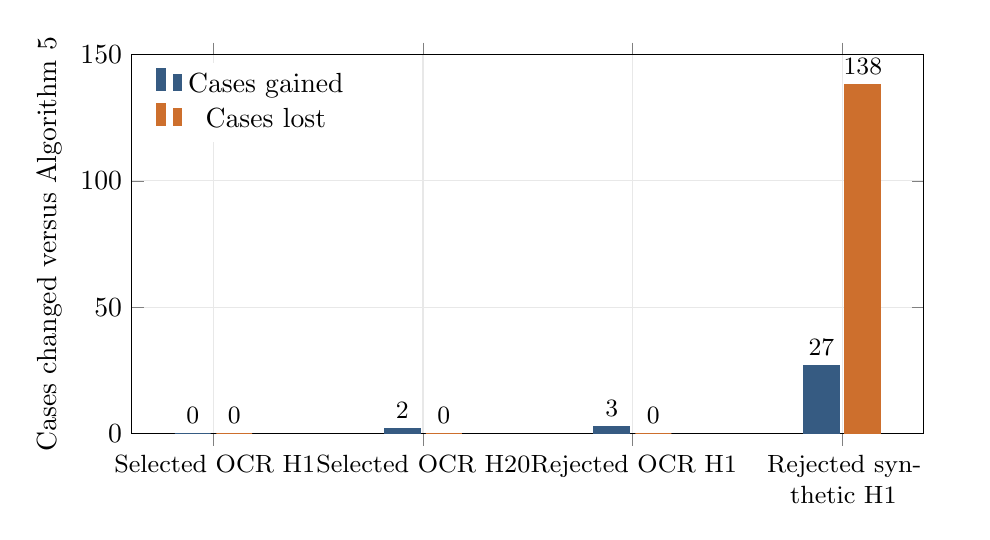
\begin{tikzpicture}
\begin{axis}[
  ybar,
  width=0.96\linewidth,
  height=6.4cm,
  ymin=0,ymax=150,
  symbolic x coords={Selected OCR H1,Selected OCR H20,Rejected OCR H1,Rejected synthetic H1},
  xtick=data,
  xticklabel style={align=center,font=\small,text width=2.8cm},
  ylabel={Cases changed versus Algorithm 5},
  bar width=13pt,
  enlarge x limits=0.13,
  grid=major,
  grid style={draw=gray!18},
  legend style={at={(0.02,0.98)},anchor=north west,legend columns=1,draw=none},
  nodes near coords,
  every node near coord/.append style={font=\small}
]
\addplot[fill=inkblue,draw=inkblue] coordinates {
  (Selected OCR H1,0) (Selected OCR H20,2)
  (Rejected OCR H1,3) (Rejected synthetic H1,27)
};
\addplot[fill=inkorange,draw=inkorange] coordinates {
  (Selected OCR H1,0) (Selected OCR H20,0)
  (Rejected OCR H1,0) (Rejected synthetic H1,138)
};
\legend{Cases gained,Cases lost}
\end{axis}
\end{tikzpicture}
\caption{The selected policy changes only OCR Hit@20 and gains two cases with
zero losses. The rejected rule would change rank 1: it gains three OCR cases,
but on the 66,257 synthetic pairs it gains 27 and loses 138. This transfer
failure is why Algorithm 6 preserves Algorithm 5's first result.}
\label{fig:paired-policy}
\end{figure}

\begin{table}[htbp]
\centering
\small
\begin{tabularx}{\linewidth}{@{}L{0.24\linewidth}Y L{0.15\linewidth}@{}}
\toprule
\textbf{Tested alternative} & \textbf{Measured result} & \textbf{Decision} \\
\midrule
Allow consensus to change rank 1 & OCR H@1 gains 3 and loses 0, but synthetic H@1 gains 27 and loses 138. Net synthetic change is $-111$ cases, or $-0.168$ percentage points. & Reject \\
Replace deterministic order with learned reranking & On the 93-family-disjoint holdout pairs, Hit@1 falls from 48.39\% to 46.24\% and Hit@20 falls from 79.57\% to 77.42\%. & Reject \\
Bounded rank-20 consensus & OCR Hit@20 gains 2 and loses 0; OCR Hit@1, Hit@5, and all synthetic top-k metrics remain unchanged. & Keep for evaluation \\
\bottomrule
\end{tabularx}
\caption{Only the bounded rank-20 change survives both OCR and synthetic paired
checks. It remains an experimental benchmark policy, not a fresh clinical validation.}
\label{tab:alternatives}
\end{table}

\FloatBarrier
\section{Failure Audit and Work Order}

P0, P1, and P2 are automated review priorities, not human verdicts. P0 means a
strong label or visible-evidence conflict. P1 means another catalog family is
one edit closer. P2 means no automated conflict was found and the supplied
target appears in the measured candidate union.

\begin{figure}[htbp]
\centering
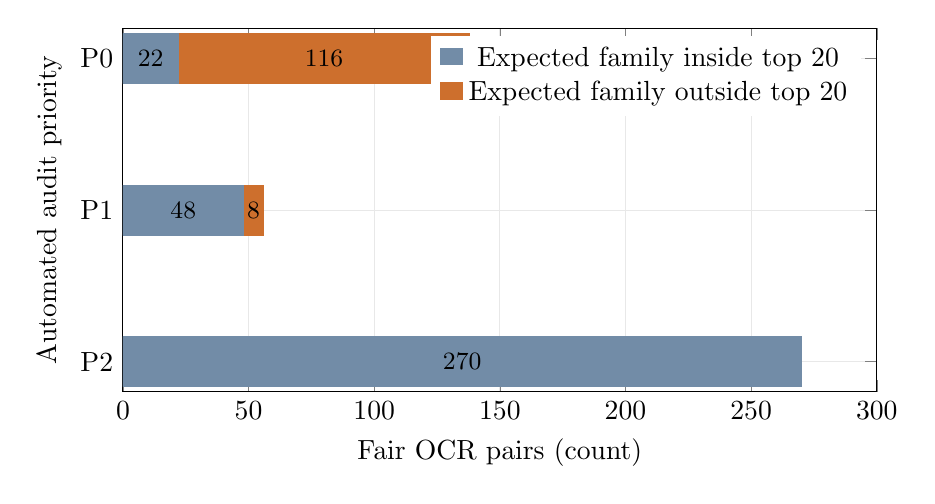
\begin{tikzpicture}
\begin{axis}[
  xbar stacked,
  width=0.92\linewidth,
  height=6.2cm,
  xmin=0,xmax=300,
  symbolic y coords={P0,P1,P2},
  ytick=data,
  y dir=reverse,
  xlabel={Fair OCR pairs (count)},
  ylabel={Automated audit priority},
  grid=major,
  grid style={draw=gray!18},
  legend style={at={(0.98,0.98)},anchor=north east,legend columns=1,draw=none},
  nodes near coords,
  every node near coord/.append style={font=\small},
  bar width=18pt
]
\addplot[fill=inkblue!70,draw=inkblue!70] coordinates {(22,P0) (48,P1) (270,P2)};
\addplot[fill=inkorange,draw=inkorange] coordinates {(116,P0) (8,P1) (0,P2)};
\legend{Expected family inside top 20,Expected family outside top 20}
\end{axis}
\end{tikzpicture}
\caption{All 124 Algorithm 6 top-20 misses are in the review queues: 116 of
138 P0 pairs and 8 of 56 P1 pairs. P2 has 270 retrieved pairs and zero misses,
but target presence in the candidate union is part of the P2 rule; this is not
an independent 100\% accuracy claim.}
\label{fig:audit}
\end{figure}

\begin{table}[H]
\centering
\small
\begin{tabularx}{\linewidth}{@{}L{0.08\linewidth}rL{0.27\linewidth}Y@{}}
\toprule
\textbf{Audit} & \textbf{Pairs} & \textbf{Example} & \textbf{Meaning and action} \\
\midrule
P0 & 138 & \code{CINNARIZIN}$\rightarrow$\code{MYOLAX}; catalog \code{CINNARIZINE} is one edit away. & Strong conflict. Check the original crop and target before changing search or using the row for learning. \\
P1 & 56 & \code{ABASCOLOGY}$\rightarrow$\code{ABASAGLAR}; \code{SPASCOLON} is one edit closer. & Borderline conflict. Keep in diagnostic metrics and send for review. \\
P2 & 270 & \code{MYMLAX}$\rightarrow$\code{MYOLAX}; the supplied family is retrieved. & Provisional clean evidence. It is eligible for cross-fitted analysis, not declared human-verified truth. \\
\bottomrule
\end{tabularx}
\caption{Every audit class is grounded by one row. None of the 464 pairs has a
linked source-image reference, so automated priority cannot replace adjudication.}
\label{tab:audit-examples}
\end{table}

Among the 124 top-20 misses, 97 supplied targets are absent from all ten source
lists. Twenty-six targets appear in only one or two lists and fail at least one
similarity rule. One target appears in four lists but fails the 55\%
Levenshtein rule. No missed target passes every gate and then loses the single
external slot; the remaining problem is missing or weak evidence, not slot
capacity.

\begin{table}[H]
\centering
\scriptsize
\setlength{\tabcolsep}{3pt}
\begin{tabularx}{\linewidth}{@{}L{0.13\linewidth}L{0.13\linewidth}L{0.14\linewidth}L{0.23\linewidth}Y@{}}
\toprule
\textbf{OCR input} & \textbf{Supplied target} & \textbf{A6 top 1} & \textbf{Expected-family evidence} & \textbf{Why it is outside top 20, and what the row shows} \\
\midrule
\code{CINNARIZIN} & \code{MYOLAX} & \code{CINNARIZINE} & 0 sources; target distance 9; nearest distance 1 & Candidate-generation miss caused by a likely label conflict. Tuning toward \code{MYOLAX} would contradict the visible text. \\
\code{H} & \code{RIVO} & no result & 0 sources; one visible character & There is not enough evidence to identify one family. Returning no result is safer than manufacturing similarity. \\
\code{HOAVACH} & \code{AMIKACIN} & \code{HYABAK} & 0 sources; target distance 6; nearest distance 3 & Severe mixed corruption removes the target from every selected list. This needs stronger retrieval or crop review, not reranking. \\
\code{LANSOPRAZOLE} & \code{LANTUS} & \code{PANTOPRAZOLE} & 1 source; Lev. 33.3\%; Jaro 81.1\% & It fails all three gate requirements. The returned family is two edits away while the supplied target is nine edits away. \\
\code{OSCAR} & \code{OSTOCAL} & \code{ASCOR} & 2 sources; Lev. 57.1\%; Jaro 83.2\% & Levenshtein passes, but source count and Jaro fail. This is a borderline P1 row where lowering one threshold is insufficient. \\
\code{RIV} & \code{RIVOTRIL} & \code{RIVO} & 2 sources; Lev. 37.5\%; Jaro 85.4\% & The prefix supports several families and an exact short family is closer. More visible letters or user confirmation are required. \\
\code{NEUROTROPHIC} & \code{NEUROCET} & \code{NEUROTOP} & 4 sources; Lev. 41.7\%; Jaro 85.0\% & Consensus and Jaro pass; only Levenshtein blocks insertion. The rule prevents four weak votes from overriding poor character agreement. \\
\code{ABACAVIR} & \code{ABASAGLAR} & \code{TECAVIR} & 1 Soundex source; Lev. 31.6\%; Jaro 65.3\% & A phonetic source alone cannot justify insertion, and \code{TECAVIR} is one edit closer than the supplied family. \\
\code{LANLTA} & \code{LANTUS} & \code{LANETAL} & 2 sources; Lev. 33.3\%; Jaro 80.6\% & The supplied family is found weakly at source ranks 18 and 20; \code{LANETAL} is one edit closer. \\
\code{TOCILIZUMAB} & \code{TOCO} & \code{ALIZOLAM} & 1 WRatio source; Lev. 27.3\%; Jaro 67.4\% & The four-letter supplied target discards most observed characters. Source-image adjudication must precede any algorithm change. \\
\bottomrule
\end{tabularx}
\caption{Ten representative Algorithm 6 top-20 failures. ``Sources'' counts
the ten ranked lists containing the supplied family. The insertion gate needs
at least three sources, Levenshtein similarity at least 55\%, and Jaro--Winkler
at least 85\%. P0 and P1 remain automated review priorities, not label verdicts.}
\label{tab:a6-ten-failures}
\end{table}

\begin{table}[H]
\centering
\small
\begin{tabularx}{\linewidth}{@{}L{0.08\linewidth}L{0.30\linewidth}Y@{}}
\toprule
\textbf{Order} & \textbf{Work item} & \textbf{Why it comes here} \\
\midrule
1 & Link source crops and adjudicate P0/P1 rows. & Every remaining top-20 miss is P0 or P1. Improving agreement with an incorrect supplied target would make the system worse. \\
2 & Keep Algorithm 5's rank 1 fixed. & The tested rank-1 rule loses 111 net synthetic cases. No measured evidence supports deploying it. \\
3 & Keep the rank-20 slot, Jaro--Winkler, BM25+, token-sort, and Dice. & These produce the only two accepted gains. Test removal of zero-delta sources on fresh reviewed cases before simplifying them. \\
4 & Reduce Algorithm 6 latency without changing output. & Mean OCR time is 48.50 ms versus 28.54 ms for Algorithm 5. Cache or parallelize independent sources and require exact rank parity. \\
5 & Run the pharmacist within-subject study. & Compare no tool, DrugEye, and Algorithm 6 on the same reviewed crops; allow ``cannot decide'' as a correct safe action. \\
\bottomrule
\end{tabularx}
\caption{The order protects label integrity first, then ranking safety,
component evidence, runtime, and finally human-use validation.}
\label{tab:priorities}
\end{table}

\end{document}
